%% —---------------------------------------------------
%% sbcreviews-en.tex
%% Template for SBC Reviews 
%% (https://journals-sol.sbc.org.br/index.php/reviews/) 
%% 
%% A versão do template inclui algumas
%% modificações sobre o template original da REIC
%% (https://journals-sol.sbc.org.br/index.php/reic)
%%
%% Licença: CCBY 4.0 
%% (https://creativecommons.org/licenses/by/4.0/)
%% Sociedade Brasileira de Computação.

\documentclass[english]{sbcreviews-2025}%

\usepackage[misc,geometry]{ifsym} 

%\usepackage{graphicx} % carregada dentro da classe
%\usepackage{fontspec} % carregada dentro da classe
%\usepackage{fontawesome} % carregada dentro da classe
%\usepackage{color} % carregada dentro da classe
%\usepackage{hyperref} % carregada dentro da classe

\usepackage{aas_macros}
\usepackage[bottom]{footmisc}

\usepackage{tabularray}
% O pacote tabularray torna o uso dos pacotes abaixo desnecessarios.
%\usepackage{supertabular}
%\usepackage{multicol}
%\usepackage{multirow}

\usepackage{afterpage}
\usepackage{url}
\usepackage{pifont}

\setcitestyle{square}

\definecolor{engtitle}{rgb}{0.5,0.5,0.5}
\definecolor{orcidlogo}{rgb}{0.37,0.48,0.13}
\definecolor{unilogo}{rgb}{0.16, 0.26, 0.58}
\definecolor{maillogo}{rgb}{0.58, 0.16, 0.26}
\definecolor{darkblue}{rgb}{0.0,0.0,0.0}
\hypersetup{colorlinks,breaklinks,
            linkcolor=darkblue,urlcolor=darkblue,
            anchorcolor=darkblue,citecolor=darkblue}
%\hypersetup{colorlinks,citecolor=blue,linkcolor=blue,urlcolor=blue}
% We disable hyperlinks by default with this line, to avoid the error "\pdfendlink ended up in different nesting level" while writing

\jid{ROCS}
\jtitle{SBC Computing Reviews, 202X, XX:1}
\issn{2966-3938}
\doi{10.5753/rocs.202X.XXXXXX}
\copyrightstatement{This work is licensed under a Creative Commons Attribution 4.0 International License}
\jyear{202X}

\category{Review}

\title[Template SBC Reviews 2025 for papers in English]{Presenting the SBC Reviews template 2025 - Version for papers in English}

%THE ORCID IS MANDATORY FOR EACH AUTHOR IN ROCS
\author[Silva et al. 202X]{
\affil{\textbf{João Silva}~\orcidlink{0000-0000-0000-0000}~\textcolor{blue}{\faEnvelope}~~[{Universidade Federal}~|\href{mailto: ...}{~{\textit{...@...br}}}~]}

\affil{\textbf{Maria Santos}~\orcidlink{0000-0000-0000-0000}~[{Universidade Federal}~|\href{mailto: ...}{~{\textit{...@...br}}}~]}

\affil{\textbf{Ana Silva }~\orcidlink{0000-0000-0000-0000}~[{Universidade Federal}~|\href{mailto: ...}{~{\textit{...@...br}}}~]}

\affil{\textbf{José Santos}~\orcidlink{0000-0000-0000-0000}~[{Universidade Federal}~|\href{mailto: ...}{~{\textit{...@...br}}}~]}

}

\begin{document}

\begin{frontmatter}

\maketitle

\begin{mail}
Institute of ..., University ..., Address, City, State, CEP, Brazil. 
\end{mail}


\begin{abstract-en}
This text, formatted as a scientific article, aims to present the new SBC paper template, describing its main features and explaining how it should be used. This version, more specifically, should be used exclusively for articles written in Portuguese that will be published in any event proceeding series at SBC OpenLib. The abstract in Portuguese, as you can see in this example, must be before the abstract in English and must have between 500 and 750 words.
\end{abstract-en}

\begin{keywords}
Proceedings, Template, SBC OpenLib, Indexing
\end{keywords}

\begin{dates}
% This information will be provided by the editor befeore publishing the paper
\noindent{\sffamily\textbf{Received:}} DD Month YYYY~~~$\bullet$~~~
{\sffamily\textbf{Accepted:}} DD Month YYYY~~~$\bullet$~~~
{\sffamily\textbf{Published:}} DD Month YYYY

\end{dates}


%\begin{license}
%Published under the Creative Commons Attribution 4.0 International Public License (CC BY 4.0)
%\end{license}

\end{frontmatter}


\section{Introduction}
\label{sec:intro}

SBC Computing Reviews — or simply SBC Reviews — is a journal published by the Brazilian Computing Society (SBC), dedicated to disseminating comprehensive and rigorous literature reviews (secondary studies) across a wide range of computing research topics. The journal welcomes various types of literature reviews frequently employed in academic research, including Systematic Literature Reviews (SLR), Multivocal Literature Reviews (MLR), Meta-Analyses, Scoping Reviews, and Systematic Mapping Studies (SMS). Additionally, updates to existing literature reviews that maintain their currency and relevance are also encouraged.

We invite authors to submit original literature reviews in either English or Portuguese. Submissions to SBC Reviews should demonstrate methodological rigor and reproducibility in the selection of original studies (primary studies), alongside thorough, high-quality analyses and clear presentation. Accepted reviews are expected to offer valuable insights by summarizing existing knowledge, identifying research gaps, and guiding future research directions – thereby contributing meaningfully to their respective domains within computing. 


Excepteur sint occaecat cupidatat non proident, sunt in culpa qui officia deserunt mollit anim id est laborum \citep{ref3}, dolor sit amet, consectetur adipiscing elit, sed do eiusmod tempor incididunt ut labore et dolore magna aliqua. Ut enim ad minim veniam, quis nostrud exercitation ullamco laboris nisi ut aliquip ex ea commodo consequat.

Lorem ipsum dolor sit amet, consectetur adipiscing elit, sed do eiusmod tempor incididunt ut labore et dolore magna aliqua. Ut enim ad minim veniam, quis nostrud exercitation ullamco laboris nisi ut aliquip ex ea commodo consequat~\citep{ref4}.
You may also use the \texttt{tabularray} package.

\begin{table}[!ht]
\caption{This is an example of table caption.}
\centering
\begin{tabular}{@{}cc@{}}
\hline\hline
Dimension & Classification accuracy \\
\hline%
 1  & 0.6232 \\
 2  & 0.9635 \\ 
 3  & 0.9724 \\ 
 4  & 0.9690 \\ 
 5  & 0.9840 \\ 
 6  & 0.9842 \\ 
 7  & 0.9873 \\ 
 8  & 0.9884 \\
 9  & 0.9873 \\ 
 10 & 0.9898 \\ 
 11 & 0.9914 \\
\hline\hline
\end{tabular}
\label{tab1}
\end{table}

\begin{table}[!ht]
\caption{This is an example of table caption.}
\centering
\begin{tblr}{%
columns={c},
row{even}={gray9},
row{1}={bg=red!10, font=\bfseries}
}
\hline
Dimension & Classification accuracy \\
\hline%
 1  & 0.6 \\
 2  & 0.963 \\
 3  & 0.97 \\
 4  & 0.9690 \\
 5  & 0.9840 \\
 6  & 0.98423 \\
 7  & 0.9873 \\
 8  & 0.9884 \\
 9  & 0.9873 \\
 10 & 0.9898 \\
 11 & 0.991 \\
\end{tblr}
\label{tab1-1}
\end{table}

Lorem ipsum dolor sit amet, consectetur adipiscing elit, sed do eiusmod tempor incididunt ut labore et dolore magna aliqua.

\section{About the Journal}

Topics of interest include, but are not limited to:

\begin{itemize}

\item Algorithms, Combinatorics, and Optimization
\item Artificial intelligence
\item Collaborative Systems
\item Computational Biology
\item Computational Intelligence
\item Computer Graphics and Image Processing
\item Computer Networks and Distributed Systems
\item Computer Ontologies
\item Computer Systems Engineering
\item Computing Applied to Health
\item Computing Education
\item Conceptual Modeling
\item Databases
\item Design of Integrated Circuits and Systems
\item Digital Games and Entertainment
\item Fault-Tolerant Systems
\item Formal Methods
\item Geoinformatics
\item Green Computing
\item High-Performance Computer Architecture and Processing
\item Human and Social Aspects in Computing
\item Human-Computer Interaction
\item Informatics in Education
\item Information and Computer Systems Security
\item Information systems
\item Multimedia and Web Systems
\item Musical Computing
\item Natural Language Processing
\item Programming Languages
\item Robotics
\item Software Engineering
\item Virtual Reality
\end{itemize}

\subsection{Publication Model}

SBC Reviews adopts a Continuous Publication model, meaning articles are published promptly after acceptance, without waiting for a full issue to be compiled. This approach accelerates the dissemination and availability of scientific findings, benefiting researchers, students, readers, publishers, and funding agencies by promoting speed and timely access to high-quality research for reading and citation.

\subsection{Diamond Open Access}

SBC Reviews is open access and free of charge for both authors and readers. All articles published by SBC Reviews are made freely and permanently accessible online immediately upon publication, without subscription charges or registration barriers. We believe the adopted policy eliminates economic and geographic barriers, fosters global democratization, and accelerates research progress. 

\subsection{Copyright Notice}
Authors publishing in SBC Reviews retain the copyright to their articles and authorize SBC to publish them under the terms of the Creative Commons Attribution 4.0 International Public License (CC BY 4.0). Thus, the authors or third parties can reproduce or distribute, in part or in whole, content extracted from the published articles, verbatim, adapted, or remixed, provided that the appropriate credits are attributed to the original authors and the original publication.

\section{Submissions}

\subsection{Submission Preparation Checklist}
As part of the submission process, authors are required to check off their submission's compliance with all of the following items. Submissions may be returned to authors who do not adhere to these guidelines.


\section{Literature Reviews}

Literature reviews are retrospective, observational studies. 
SBC Reviews publishes literature reviews in Computing research fields, including but not limited to the following review types:

\textbf{Systematic literature reviews} (SLR) are rigorous, comprehensive reviews aimed at answering a specific, focused research question by critically appraising and synthesizing all relevant original research studies. If statistical methods are used to combine quantitative data from  multiple studies, it is a Meta Analysis study.

\textbf{Multivocal literature reviews} (MLR) are a type of SLR that incorporates both formal, peer-reviewed literature (like journal articles and conference papers) and grey literature. Grey literature includes materials such as technical reports, blog posts, and conference presentations, which may not be formally published or peer-reviewed. 

\textbf{Scoping reviews} (SCR) address broader, exploratory research questions to map the extent, range, and nature of research on a particular topic. Among other objectives, scoping reviews help determine whether a systematic review of the literature is necessary.

\textbf{Systematic mapping studies} (SMS) focus on categorizing and quantifying existing literature to provide an overview of research activity in a subfield.

SBC Reviews also appraises submissions of literature reviews that address evaluations of progress and/or critical assessments relevant to specific subfields.


%\subsection{What Is Eligibility Criteria In A Systematic Review?}
%Source: \url{https://www.distillersr.com/resources/systematic-literature-reviews/eligibility-criteria-in-a-systematic-review}

%Eligibility criteria is a pre-specified, unambiguous basis that determines the scope of studies to be synthesized in a systematic review. The eligibility criteria can be developed newly by the authors, or it can be adopted from another review. In the second scenario, the original authors must be referenced. It guides the selection of literature during the search in databases or other sources. During title, abstract or full-text reading, or potential articles, the criteria dictates what must be included (inclusion criteria), and excluded (exclusion criteria) in the review. These are a fundamental prerequisite of all systematic review methods and are often recorded as a paragraph, or table within the methodology section of the final report.
% Eligibility criteria are defined after setting the research question, and study objective(s), and before data collection. However, scoping searches may be performed beforehand to better establish them.
 
\section{Example of Head Level 1}
Lorem ipsum dolor sit amet, consectetur adipiscing elit, sed do eiusmod tempor incididunt ut labore et dolore magna aliqua. Ut enim ad minim veniam, quis nostrud exercitation ullamco laboris nisi ut aliquip ex ea commodo consequat. Duis aute irure dolor in reprehenderit in voluptate velit esse cillum dolore eu fugiat nulla pariatur. Excepteur sint occaecat cupidatat non proident, sunt in culpa qui officia deserunt mollit anim id est laborum. Lorem ipsum dolor sit amet, consectetur adipiscing elit, sed do eiusmod tempor incididunt ut labore et dolore magna aliqua. Ut enim ad minim veniam, quis nostrud exercitation ullamco laboris nisi ut aliquip ex ea commodo consequat. Duis aute irure dolor in reprehenderit in voluptate velit esse cillum dolore eu fugiat nulla pariatur. Excepteur sint occaecat cupidatat non proident, sunt in culpa qui officia deserunt mollit anim id est laborum.

\subsection{This is an example of head level 2}

Lorem ipsum dolor sit amet, consectetur adipiscing elit, sed do eiusmod tempor incididunt ut labore et dolore magna aliqua. Ut enim ad minim veniam, quis nostrud exercitation ullamco laboris nisi ut aliquip ex ea commodo consequat. Duis aute irure dolor in reprehenderit in voluptate velit esse cillum dolore eu fugiat nulla pariatur. Excepteur sint occaecat cupidatat non proident, sunt in culpa qui officia deserunt mollit anim id est laborum.

\begin{quotation}
\textit{This is a longer quotation. Lorem ipsum dolor sit amet, consectetur adipiscing elit, sed do eiusmod tempor incididunt ut labore et dolore magna aliqua. Lorem ipsum dolor sit amet, consectetur adipiscing elit, sed do eiusmod tempor incididunt ut labore et magna aliqua. 
}\end{quotation} 

\subsubsection{This is an example of head level 3}
Lorem ipsum dolor sit amet, consectetur adipiscing elit, sed do eiusmod tempor incididunt ut labore et dolore magna aliqua. Ut enim ad minim veniam, quis nostrud exercitation ullamco laboris nisi ut aliquip ex ea commodo consequat. Duis aute irure dolor in reprehenderit in voluptate velit esse cillum dolore eu fugiat nulla pariatur. Excepteur sint occaecat cupidatat non proident, sunt in culpa qui officia deserunt mollit anim id est laborum. Lorem ipsum dolor sit amet, consectetur adipiscing elit, sed do eiusmod tempor incididunt ut labore et dolore magna aliqua. Ut enim ad minim veniam, quis nostrud exercitation ullamco laboris nisi ut aliquip ex ea commodo consequat. Duis aute irure dolor in reprehenderit in voluptate velit esse cillum dolore eu fugiat nulla pariatur. Excepteur sint occaecat cupidatat non proident, sunt in culpa qui officia deserunt mollit anim id est laborum.

\paragraph{This is an example of head level 4.}
Lorem ipsum dolor sit amet, consectetur adipiscing elit, sed do eiusmod tempor incididunt ut labore et dolore magna aliqua. Ut enim ad minim veniam, quis nostrud exercitation ullamco laboris nisi ut aliquip ex ea commodo consequat. Duis aute irure dolor in reprehenderit in voluptate velit esse cillum dolore eu fugiat nulla pariatur. Excepteur sint occaecat cupidatat non proident, sunt in culpa qui officia deserunt mollit anim id est laborum. 
Let
\[
x=(x_1,\dots,x_n)\in R^n
\]be an \(n\)-dimensional vector. The sparse PCA problem can be written as
\begin{equation}\label{eq1}
\max\limits_{x}\{x^TAx-\rho\|x\|_0:x^Tx=1\},
\end{equation}
Lorem ipsum dolor sit amet, consectetur adipiscing elit, sed do eiusmod tempor incididunt ut labore et dolore magna aliqua. Ut enim ad minim veniam, quis nostrud exercitation ullamco laboris nisi ut aliquip ex ea commodo consequat. Duis aute irure dolor in reprehenderit in voluptate velit esse cillum dolore eu fugiat nulla pariatur\break equation (\ref{eq1}). 
\[\max\limits_{x}\{x^TAx :x^Tx=1\}.\]
If $A$ Lorem ipsum dolor sit amet, consectetur adipiscing elit, sed do eiusmod tempor incididunt ut labore et dolore magna aliqua. Ut enim ad minim veniam, quis nostrud exercitation ullamco laboris nisi ut aliquip ex ea commodo consequat. 


Equation (\ref{eq1}) is a special case of the following sparse generalized eigenvector problem (GEV):
\begin{equation}\label{GEV}
\max\limits_{x}\{x^TAx-\rho \|x\|_0: x^TBx\leq 1\},
\end{equation}

Lorem ipsum dolor sit amet, consectetur adipiscing elit, sed do eiusmod tempor incididunt ut labore et dolore magna aliqua. Ut enim ad minim veniam, quis nostrud exercitation ullamco laboris nisi ut aliquip ex ea commodo consequat. Duis aute irure dolor in reprehenderit in voluptate velit esse cillum dolore eu fugiat nulla pariatur. Excepteur sint occaecat cupidatat non proident, sunt in culpa qui officia deserunt mollit anim id est laborum. 

Lorem ipsum dolor sit amet, consectetur adipiscing elit, sed do eiusmod tempor incididunt ut labore et dolore magna aliqua. Ut enim ad minim veniam, quis nostrud exercitation ullamco laboris nisi ut aliquip ex ea commodo consequat. Duis aute irure dolor in reprehenderit in voluptate velit esse cillum dolore eu fugiat nulla pariatur. Excepteur sint occaecat cupidatat non proident, sunt in culpa qui officia deserunt mollit anim id est laborum \textbf{Table~\ref{tab2}}.

\section{Example of Head Level 1}

Lorem ipsum dolor sit amet, consectetur adipiscing elit, sed do eiusmod tempor incididunt ut labore et dolore magna aliqua. Ut enim ad minim veniam, quis nostrud exercitation ullamco laboris nisi ut aliquip ex ea commodo consequat. Duis aute irure dolor in reprehenderit in voluptate velit esse cillum dolore eu fugiat nulla pariatur. Excepteur sint occaecat cupidatat non proident, sunt in culpa qui officia deserunt mollit anim id est laborum. Lorem ipsum dolor sit amet, consectetur adipiscing elit, sed do eiusmod tempor incididunt ut labore et dolore magna aliqua. Ut enim ad minim veniam, quis nostrud exercitation ullamco laboris nisi ut aliquip ex ea commodo consequat. Duis aute irure dolor in reprehenderit in voluptate velit esse cillum dolore eu fugiat nulla pariatur. Excepteur sint occaecat cupidatat non proident, sunt in culpa qui officia deserunt mollit anim id est laborum.


\begin{table*}
\caption{It is rather for us to be here dedicated to the great $\alpha^{(1)}$ and $\alpha^{(2)}$ task remaining before us  that from these honoured dead we take increased devotion to that cause for which they here gave the last.} 
\centering
\begin{tabular*}{\textwidth}{@{}c\x c\x c\x c\x c\x c\x c\x c\x c\x c\x c\x c@{}}
\hline \hline
 Layer   & $V_{\rm P0}$   & $V_{\rm S0}$     &  $\epsilon^{(1)}$  &  $\epsilon^{(2)}$ 
         & $\delta^{(1)}$ & $\delta^{(2)}$  &  $\delta^{(3)}$    & $\gamma^{(1)}$ 
         & $\gamma^{(2)}$ & $\alpha^{(1)}$  & $\alpha^{(2)}$ \\
 number  & (km/s)        & (km/s)          & ~                  & ~ 
         & ~             & ~               & ~                  & ~ 
         & ~             & $(^\circ)$       & $(^\circ)$ \\
%
\hline
 1 & 3.5 & 2.0 & 0.20 & -0.05 & 0.00 & -0.20 & -0.05 & 0.20 & ~0.05 & 20 & 10 \\ 
 2 & 2.5 & 1.5 & 0.10 & -0.15 & 0.05 & -0.15 & ~0.00 & 0.10 & -0.05 & 20 & 40 \\ 
 3 & 3.0 & 1.8 & 0.20 & -0.05 & 0.25 & ~0.05 & ~0.20 & 0.15 & ~0.00 & 20 & 70$^a$ \\
\hline \hline
\end{tabular*}\label{tab2}
\end{table*}

Lorem ipsum dolor sit amet, consectetur adipiscing elit, sed do eiusmod tempor incididunt ut labore et dolore magna aliqua. Ut enim ad minim veniam, quis nostrud exercitation ullamco laboris nisi ut aliquip ex ea commodo consequat. Duis aute irure dolor in reprehenderit in voluptate velit esse cillum dolore eu fugiat nulla pariatur. Excepteur sint occaecat cupidatat non proident, sunt in culpa qui officia deserunt mollit anim id est laborum. Lorem ipsum dolor sit amet, consectetur adipiscing elit, sed do eiusmod tempor incididunt ut labore et dolore magna aliqua. Ut enim ad minim veniam, quis nostrud exercitation ullamco laboris nisi ut aliquip ex ea commodo consequat. Duis aute irure dolor in reprehenderit in voluptate velit esse cillum dolore eu fugiat nulla pariatur. Excepteur sint occaecat cupidatat non proident, sunt in culpa qui officia deserunt mollit anim id est laborum.

\begin{itemize}
\item This is a longer itemize list. It consists of two paragraphs of text, neither of which are particularly interesting {\sc ii}.
\item This is a longer itemize list. It consists of two paragraphs of text, neither of which are particularly interesting.
\item This is a longer itemize list. It consists of two paragraphs of text, neither of which are particularly interesting.
\end{itemize}

Lorem ipsum dolor sit amet, consectetur adipiscing elit, sed do eiusmod tempor incididunt ut labore et dolore magna aliqua. Ut enim ad minim veniam, quis nostrud exercitation ullamco laboris nisi ut aliquip ex ea commodo consequat. Duis aute irure dolor in reprehenderit in voluptate velit esse cillum dolore eu fugiat nulla pariatur. Excepteur sint occaecat cupidatat non proident, sunt in culpa qui officia deserunt mollit anim id est laborum. Lorem ipsum dolor sit amet, consectetur adipiscing elit, sed do eiusmod tempor incididunt ut labore et dolore magna aliqua. Ut enim ad minim veniam, quis nostrud exercitation ullamco laboris nisi ut aliquip ex ea commodo consequat. Duis aute irure dolor in reprehenderit in voluptate velit esse cillum dolore eu fugiat nulla pariatur. Excepteur sint occaecat cupidatat non proident, sunt in culpa qui officia deserunt mollit anim id est laborum.

\begin{enumerate}%
\item This is a longer numbered list. It consists of two paragraphs of text, neither of which are particularly interesting.
\item This is a short numbered list. It consists of two paragraphs of text.
\end{enumerate}

Lorem ipsum dolor sit amet, consectetur adipiscing elit, sed do eiusmod tempor incididunt ut labore et dolore magna aliqua. Ut enim ad minim veniam, quis nostrud exercitation ullamco laboris nisi ut aliquip ex ea commodo consequat. Duis aute irure dolor in reprehenderit in voluptate velit esse cillum dolore eu fugiat nulla pariatur. Excepteur sint occaecat cupidatat non proident, sunt in culpa qui officia deserunt mollit anim id est laborum. Lorem ipsum dolor sit amet, consectetur adipiscing elit, sed do eiusmod tempor incididunt ut labore et dolore magna aliqua. Ut enim ad minim veniam, quis nostrud exercitation ullamco laboris nisi ut aliquip ex ea commodo consequat. Duis aute irure dolor in reprehenderit in voluptate velit esse cillum dolore eu fugiat nulla pariatur. Excepteur sint occaecat cupidatat non proident, sunt in culpa qui officia deserunt mollit anim id est laborum.

Lorem ipsum dolor sit amet, consectetur adipiscing elit, sed do eiusmod tempor incididunt ut labore et dolore magna aliqua. Ut enim ad minim veniam, quis nostrud exercitation ullamco laboris nisi ut aliquip ex ea commodo consequat. Duis aute irure dolor in reprehenderit in voluptate velit esse cillum dolore eu fugiat nulla pariatur. Excepteur sint occaecat cupidatat non proident, sunt in culpa qui officia deserunt mollit anim id est laborum. Lorem ipsum dolor sit amet, consectetur adipiscing elit, sed do eiusmod tempor incididunt ut labore et dolore magna aliqua. Ut enim ad minim veniam, quis nostrud exercitation ullamco laboris nisi ut aliquip ex ea commodo consequat. Duis aute irure dolor in reprehenderit in voluptate velit esse cillum dolore eu fugiat nulla pariatur. Excepteur sint occaecat cupidatat non proident, sunt in culpa qui officia deserunt mollit anim id est laborum.


\subsection{This is an example of head level 2}

Lorem ipsum dolor sit amet, consectetur adipiscing elit, sed do eiusmod tempor incididunt ut labore et dolore magna aliqua. Ut enim ad minim veniam, quis nostrud exercitation ullamco laboris nisi ut aliquip ex ea commodo consequat. Duis aute irure dolor in reprehenderit in voluptate velit esse cillum dolore eu fugiat nulla pariatur. Excepteur sint occaecat cupidatat non proident, sunt in culpa qui officia deserunt mollit anim id est laborum. Lorem ipsum dolor sit amet, consectetur adipiscing elit, sed do eiusmod tempor incididunt ut labore et dolore magna aliqua. Ut enim ad minim veniam, quis nostrud exercitation ullamco laboris nisi ut aliquip ex ea commodo consequat. Duis aute irure dolor in reprehenderit in voluptate velit esse cillum dolore eu fugiat nulla pariatur. Excepteur sint occaecat cupidatat non proident, sunt in culpa qui officia deserunt mollit anim id est laborum \textbf{Figure \ref{Fig1}}.

Lorem ipsum dolor sit amet, consectetur adipiscing elit, sed do eiusmod tempor incididunt ut labore et dolore magna aliqua. Ut enim ad minim veniam, quis nostrud exercitation ullamco laboris nisi ut aliquip ex ea commodo consequat. Duis aute irure dolor in reprehenderit in voluptate velit esse cillum dolore eu fugiat nulla pariatur. Excepteur sint occaecat cupidatat non proident, sunt in culpa qui officia deserunt mollit anim id est laborum. Lorem ipsum dolor sit amet, consectetur adipiscing elit, sed do eiusmod tempor incididunt ut labore et dolore magna aliqua. Ut enim ad minim veniam, quis nostrud exercitation ullamco laboris nisi ut aliquip ex ea commodo consequat. Duis aute irure dolor in reprehenderit in voluptate velit esse cillum dolore eu fugiat nulla pariatur. Excepteur sint occaecat cupidatat non proident, sunt in culpa qui officia deserunt mollit anim id est laborum.

Lorem ipsum dolor sit amet, consectetur adipiscing elit, sed do eiusmod tempor incididunt ut labore et dolore magna aliqua. Ut enim ad minim veniam, quis nostrud exercitation ullamco laboris nisi ut aliquip ex ea commodo consequat. Duis aute irure dolor in reprehenderit in voluptate velit esse cillum dolore eu fugiat nulla pariatur. Excepteur sint occaecat cupidatat non proident, sunt in culpa qui officia deserunt mollit anim id est laborum. Lorem ipsum dolor sit amet, consectetur adipiscing elit, sed do eiusmod tempor incididunt ut labore et dolore magna aliqua. Ut enim ad minim veniam, quis nostrud exercitation ullamco laboris nisi ut aliquip ex ea commodo consequat. Duis aute irure dolor in reprehenderit in voluptate velit esse cillum dolore eu fugiat nulla pariatur. Excepteur sint occaecat cupidatat non proident, sunt in culpa qui officia deserunt mollit anim id est laborum.

\begin{figure}
\begin{center}
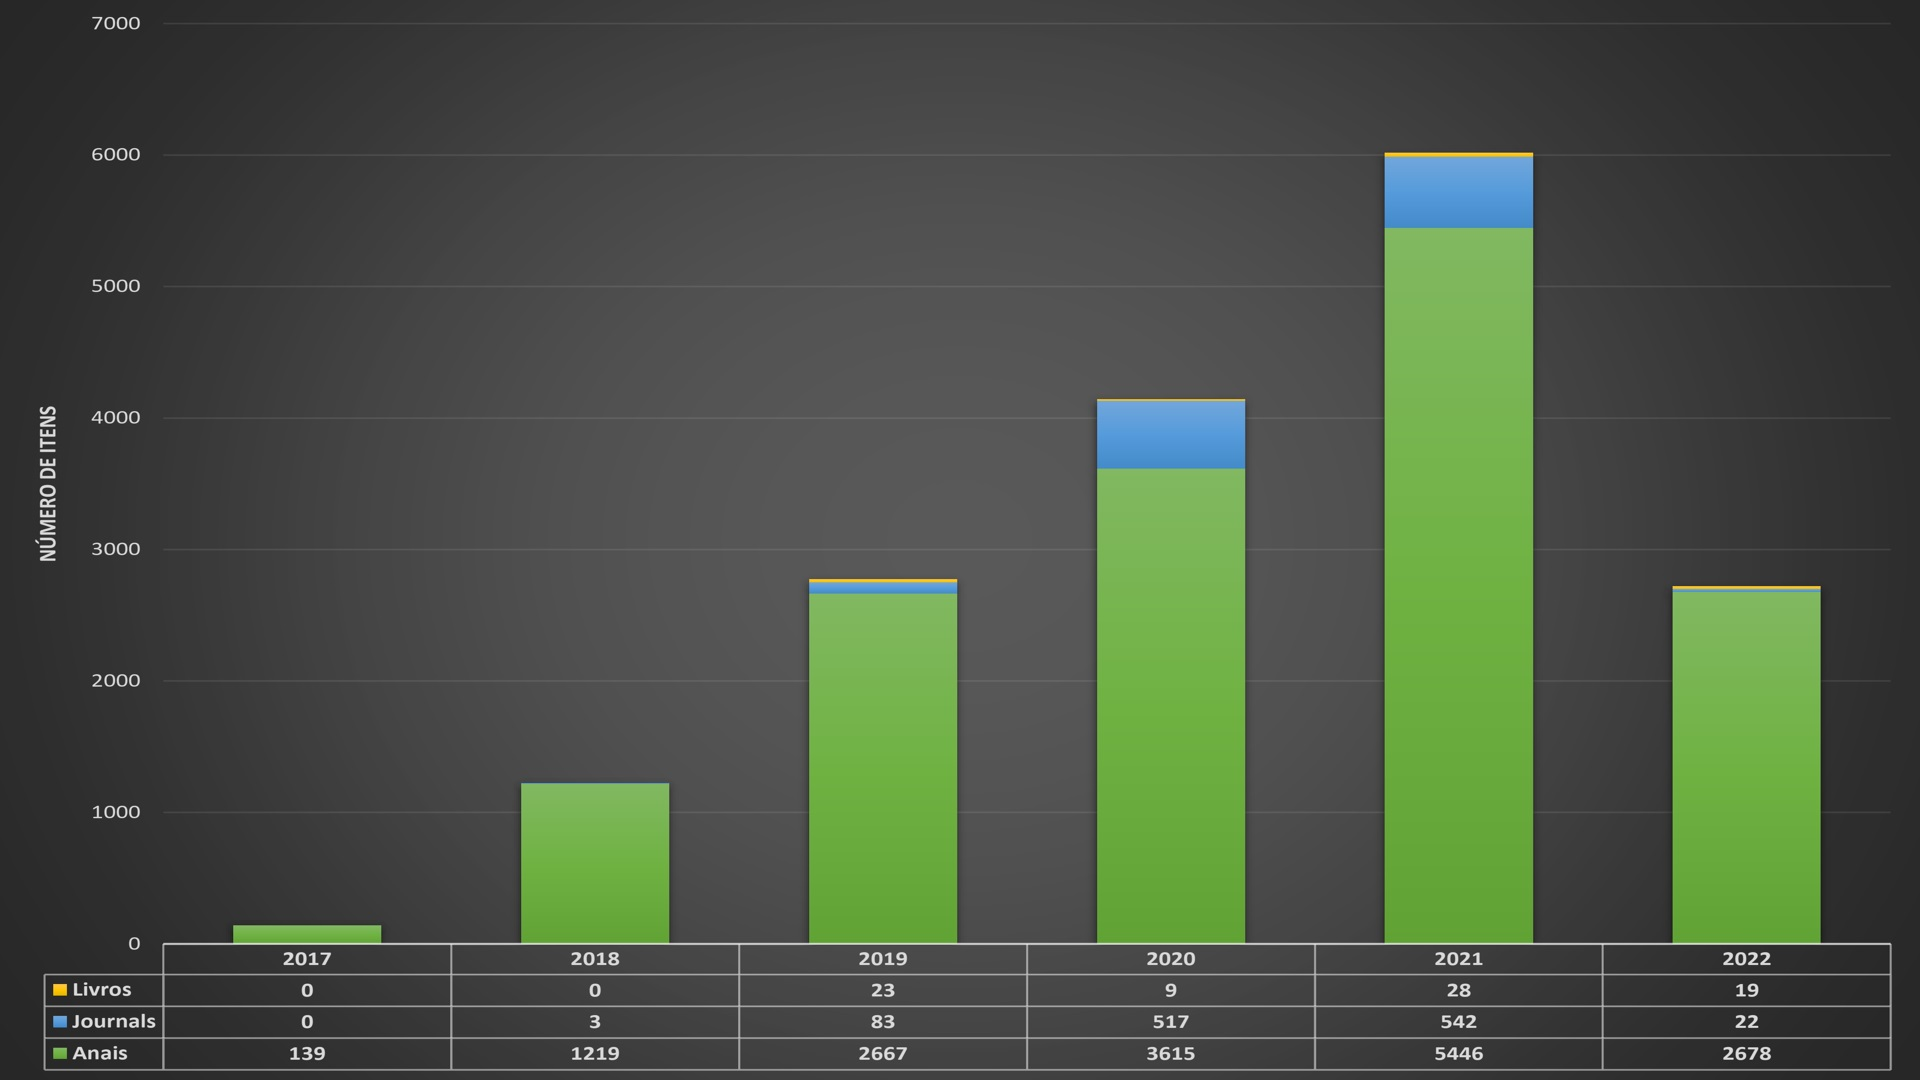
\includegraphics[width=\columnwidth]{sol.jpg}
\caption{This is an example of figure caption.}\label{Fig1}
\end{center}
\end{figure}

Lorem ipsum dolor sit amet, consectetur adipiscing elit, sed do eiusmod tempor incididunt ut labore et dolore magna aliqua. Ut enim ad minim veniam, quis nostrud exercitation ullamco laboris nisi ut aliquip ex ea commodo consequat. Duis aute irure dolor in reprehenderit in voluptate velit esse cillum dolore eu fugiat nulla pariatur. Excepteur sint occaecat cupidatat non proident, sunt in culpa qui officia deserunt mollit anim id est laborum. Lorem ipsum dolor sit amet, consectetur adipiscing elit, sed do eiusmod tempor incididunt ut labore et dolore magna aliqua. Ut enim ad minim veniam, quis nostrud exercitation ullamco laboris nisi ut aliquip ex ea commodo consequat. Duis aute irure dolor in reprehenderit in voluptate velit esse cillum dolore eu fugiat nulla pariatur. Excepteur sint occaecat cupidatat non proident, sunt in culpa qui officia deserunt mollit anim id est laborum \textbf{Figure \ref{Fig2}}.

Lorem ipsum dolor sit amet, consectetur adipiscing elit, sed do eiusmod tempor incididunt ut labore et dolore magna aliqua. Ut enim ad minim veniam, quis nostrud exercitation ullamco laboris nisi ut aliquip ex ea commodo consequat. Duis aute irure dolor in reprehenderit in voluptate velit esse cillum dolore eu fugiat nulla pariatur. Excepteur sint occaecat cupidatat non proident, sunt in culpa qui officia deserunt mollit anim id est laborum. Lorem ipsum dolor sit amet, consectetur adipiscing elit, sed do eiusmod tempor incididunt ut labore et dolore magna aliqua. Ut enim ad minim veniam, quis nostrud exercitation ullamco laboris nisi ut aliquip ex ea commodo consequat. Duis aute irure dolor in reprehenderit in voluptate velit esse cillum dolore eu fugiat nulla pariatur. Excepteur sint occaecat cupidatat non proident, sunt in culpa qui officia deserunt mollit anim id est laborum.

\begin{figure*}
\begin{center}
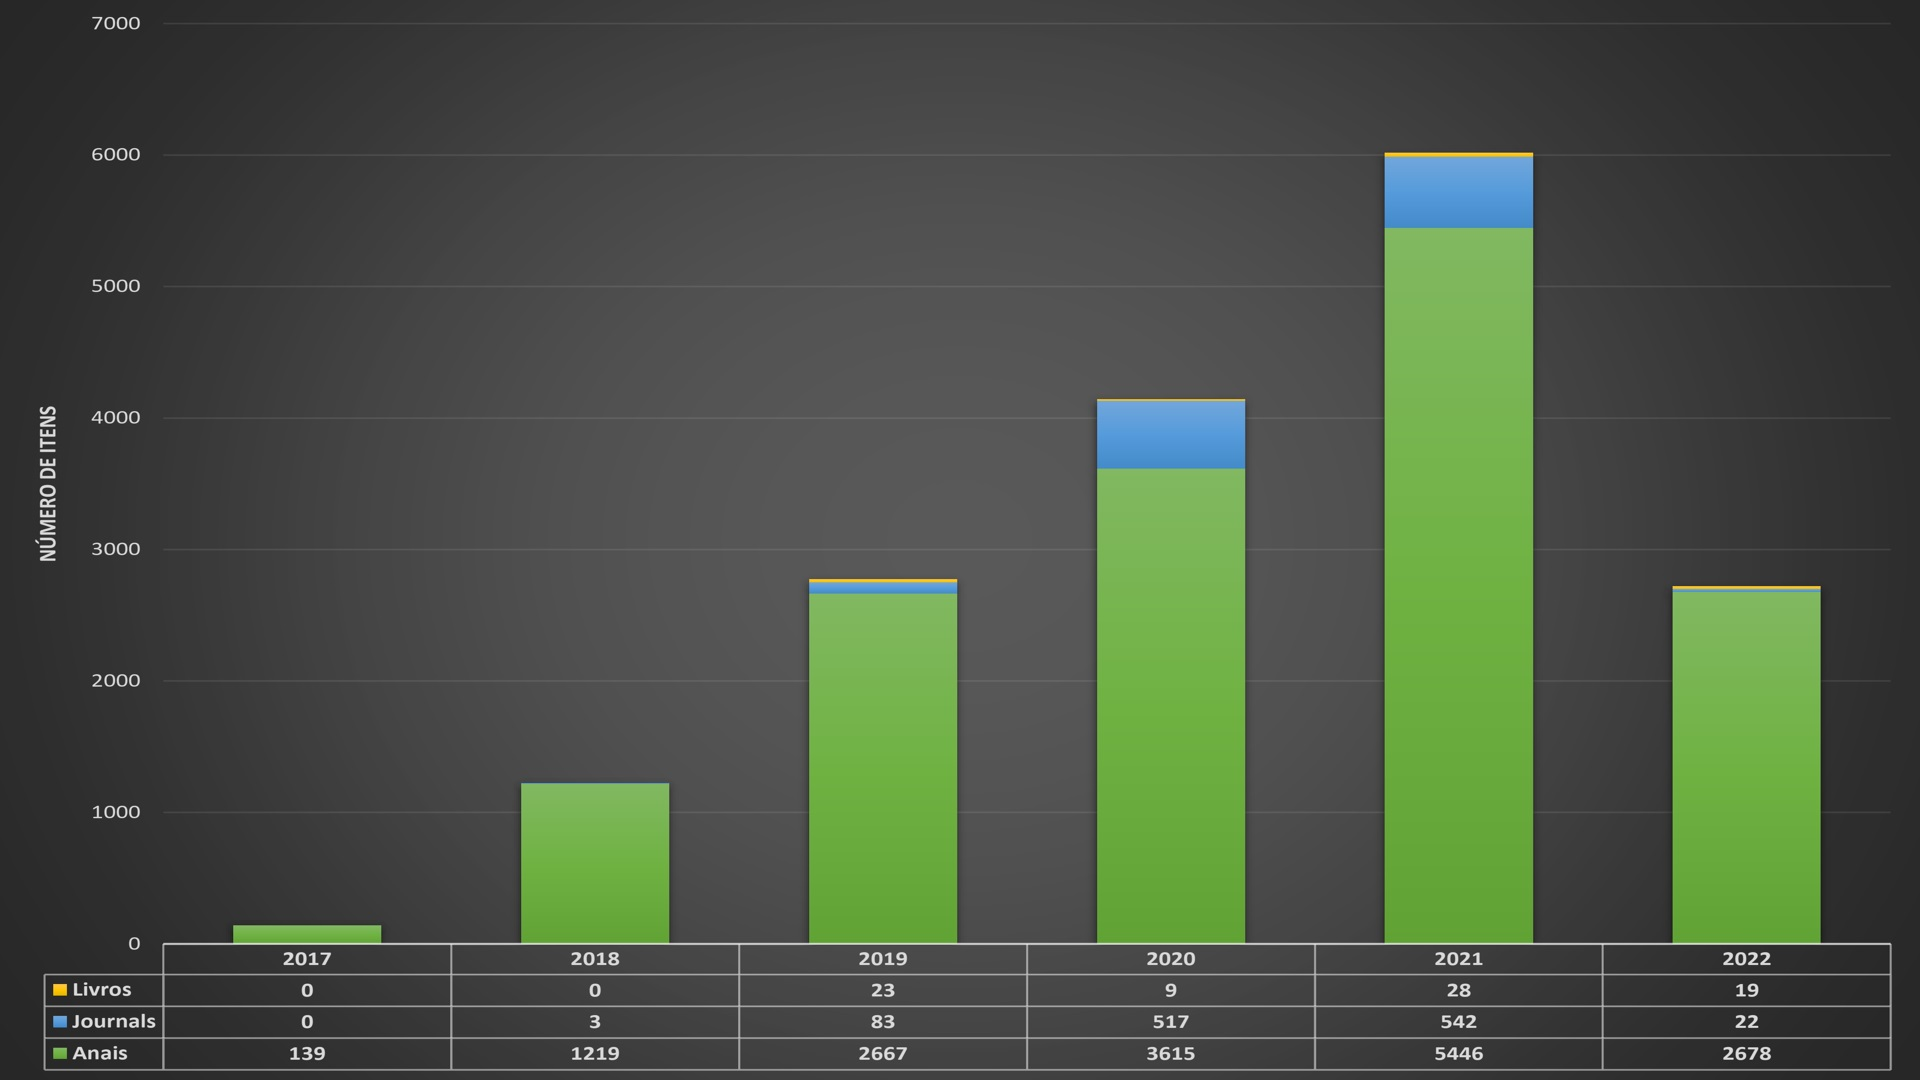
\includegraphics[width=30pc]{sol.jpg}
\caption{{This is an example of figure caption.}}
 \label{Fig2}
\end{center}
\end{figure*}

Lorem ipsum dolor sit amet, consectetur adipiscing elit, sed do eiusmod tempor incididunt ut labore et dolore magna aliqua. Ut enim ad minim veniam, quis nostrud exercitation ullamco laboris nisi ut aliquip ex ea commodo consequat. Duis aute irure dolor in reprehenderit in voluptate velit esse cillum dolore eu fugiat nulla pariatur. Excepteur sint occaecat cupidatat non proident, sunt in culpa qui officia deserunt mollit anim id est laborum. Lorem ipsum dolor sit amet, consectetur adipiscing elit, sed do eiusmod tempor incididunt ut labore et dolore magna aliqua. Ut enim ad minim veniam, quis nostrud exercitation ullamco laboris nisi ut aliquip ex ea commodo consequat. Duis aute irure dolor in reprehenderit in voluptate velit esse cillum dolore eu fugiat nulla pariatur. Excepteur sint occaecat cupidatat non proident, sunt in culpa qui officia deserunt mollit anim id est laborum.

Lorem ipsum dolor sit amet, consectetur adipiscing elit, sed do eiusmod tempor incididunt ut labore et dolore magna aliqua. Ut enim ad minim veniam, quis nostrud exercitation ullamco laboris nisi ut aliquip ex ea commodo consequat. Duis aute irure dolor in reprehenderit in voluptate velit esse cillum dolore eu fugiat nulla pariatur. Excepteur sint occaecat cupidatat non proident, sunt in culpa qui officia deserunt mollit anim id est laborum. Lorem ipsum dolor sit amet, consectetur adipiscing elit, sed do eiusmod tempor incididunt ut labore et dolore magna aliqua. Ut enim ad minim veniam, quis nostrud exercitation ullamco laboris nisi ut aliquip ex ea commodo consequat. Duis aute irure dolor in reprehenderit in voluptate velit esse cillum dolore eu fugiat nulla pariatur. Excepteur sint occaecat cupidatat non proident, sunt in culpa qui officia deserunt mollit anim id est laborum.



\paragraph{This is an example of head level 4.}

Excepteur sint occaecat cupidatat non proident, sunt in culpa qui officia deserunt mollit anim id est laborum. Lorem ipsum dolor sit amet, consectetur adipiscing elit, sed do eiusmod tempor incididunt ut labore et dolore magna aliqua. Ut enim ad minim veniam, quis nostrud exercitation ullamco laboris nisi ut aliquip ex ea commodo consequat. Duis aute irure dolor in reprehenderit in voluptate velit esse cillum dolore eu fugiat nulla pariatur. 

Lorem ipsum dolor sit amet, consectetur adipiscing elit, sed do eiusmod tempor incididunt ut labore et dolore magna aliqua. Ut enim ad minim veniam, quis nostrud exercitation ullamco laboris nisi ut aliquip ex ea commodo consequat. Excepteur sint occaecat cupidatat non proident, sunt in culpa qui officia deserunt mollit anim id est laborum. Lorem ipsum dolor sit amet, consectetur adipiscing elit, sed do eiusmod tempor incididunt ut labore et dolore magna aliqua. Ut enim ad minim veniam, quis nostrud exercitation ullamco laboris nisi ut aliquip ex ea commodo consequat. Duis aute irure dolor in reprehenderit in voluptate velit esse cillum dolore eu fugiat nulla pariatur. Excepteur sint occaecat cupidatat non proident, sunt in culpa qui officia deserunt mollit anim id est laborum.

\section{Conclusion}

Excepteur sint occaecat cupidatat non proident, sunt in culpa qui officia deserunt mollit anim id est laborum. Lorem ipsum dolor sit amet, consectetur adipiscing elit, sed do eiusmod tempor incididunt ut labore et dolore magna aliqua. Ut enim ad minim veniam, quis nostrud exercitation ullamco laboris nisi ut aliquip ex ea commodo consequat. Duis aute irure dolor in reprehenderit in voluptate velit esse cillum dolore eu fugiat nulla pariatur. 

Ut enim ad minim veniam, quis nostrud exercitation ullamco laboris nisi ut aliquip ex ea commodo consequat. Duis aute irure dolor in reprehenderit in voluptate velit esse cillum dolore eu fugiat nulla pariatur. Excepteur sint occaecat cupidatat non proident, sunt in culpa qui officia deserunt mollit anim id est laborum \citep{ref5}.


\begin{declarations}

\begin{acknowledgements}
THIS DECLARATION IS OPTIONAL. 
This is a multiline text of acknowledgments. 
Lorem ipsum dolor sit amet, consectetur adipiscing elit, 
sed do eiusmod tempor incididunt ut labore et dolore magna aliqua. 
Ut enim ad minim veniam, quis nostrud exercitation ullamco laboris nisi ut aliquip ex ea commodo consequat.
\end{acknowledgements}

\begin{funding}
THIS DECLARATION IS OPTIONAL. This research was funded by lorem ipsum dolor sit amet, consectetur adipiscing elit.
\end{funding}

\begin{contributions}
THIS DECLARATION IS MANDATORY. 
\textit{Consider the SBC Code of Conduct.
Participation in authorship: All authors of a published work
or submitted for publication are expected to have actively participated in the respective work.}
We suggest that authors describe their contribution using
the CRediT Taxonomy (\href{https://credit.niso.org/}{https://credit.niso.org/}) as in this example:
JV contributed to the design of this study. CB, RP, and CM performed the experiments.
JV is the primary contributor and writer of this manuscript.
All authors read and approved the final manuscript.
\end{contributions}

\begin{interests}
THIS DECLARATION IS MANDATORY. If there are no competing interests, the authors should declare: ``The authors declare that they have no competing interests''. Otherwise, the declaration should be: ``The authors declare that they have the following competing interests, lorem ipsum dolor sit amet, consectetur adipiscing elit.''
\end{interests}

\begin{materials}
THIS DECLARATION IS MANDATORY. 
\textit{Consider the SBC Code of Conduct.
Reproducibility of research results:
Where applicable, it is recommended that articles indicate
the public availability of material used in the reviews,
to facilitate the reproduction of the respective results by other researchers.}
%
If the authors have made their data and/or code publicly available, the statement should read:
``The data and other materials created and/or used in this literature review
are available at \ldots''.
Otherwise, the statement should read:
``The data and other materials created and/or used in this literature review
will be made available upon request''.
%
All supplementary material made publicly available by the authors will appear
on the article's publication page if accepted.
\end{materials}

\begin{aitools}
THIS DECLARATION IS MANDATORY. 
\textit{Consider the SBC Code of Conduct.
Use of Generative Artificial Intelligence (AI):
The use of generative AI tools and technologies for content generation,
in writing and/or reviewing the content of articles, must be explicitly declared in the paper.}
The declaration should appear in this section, specifically defined for this purpose.
The tools (and their versions) should be listed and where they were used, for example,
texts, tables, graphs, citations, etc.
These tools \textbf{may not} be listed as authors of an article.
The use of such tools does not exempt the authors from responsibility
for all of their content, including if plagiarism is identified.
%
If the authors did not use such tools, the statement should be:
``The authors did not use generative AI tools in the development of the study.''
\end{aitools}

\begin{furtherinformation}
Manuscripts must explicitly 
\textbf{indicate how the ethical issues of the research were addressed and managed}, 
including the research approval by an ethics committee when applicable. 
\end{furtherinformation}

\end{declarations}

\bibliographystyle{apalike-sol}
\bibliography{refs}

\end{document}
